%Version 3 October 2023
% See section 11 of the User Manual for version history
%
%%%%%%%%%%%%%%%%%%%%%%%%%%%%%%%%%%%%%%%%%%%%%%%%%%%%%%%%%%%%%%%%%%%%%%
%%                                                                 %%
%% Please do not use \input{...} to include other tex files.       %%
%% Submit your LaTeX manuscript as one .tex document.              %%
%%                                                                 %%
%% All additional figures and files should be attached             %%
%% separately and not embedded in the \TeX\ document itself.       %%
%%                                                                 %%
%%%%%%%%%%%%%%%%%%%%%%%%%%%%%%%%%%%%%%%%%%%%%%%%%%%%%%%%%%%%%%%%%%%%%

%%\documentclass[referee,sn-basic]{sn-jnl}% referee option is meant for double line spacing

%%=======================================================%%
%% to print line numbers in the margin use lineno option %%
%%=======================================================%%

\documentclass[lineno,sn-basic]{sn-jnl}% Basic Springer Nature Reference Style/Chemistry Reference Style

%%======================================================%%
%% to compile with pdflatex/xelatex use pdflatex option %%
%%======================================================%%

%%\documentclass[pdflatex,sn-basic]{sn-jnl}% Basic Springer Nature Reference Style/Chemistry Reference Style


%%Note: the following reference styles support Namedate and Numbered referencing. By default the style follows the most common style. To switch between the options you can add or remove “Numbered” in the optional parenthesis. 
%%The option is available for: sn-basic.bst, sn-vancouver.bst, sn-chicago.bst%  
 
%%\documentclass[sn-nature]{sn-jnl}% Style for submissions to Nature Portfolio journals
%%\documentclass[sn-basic]{sn-jnl}% Basic Springer Nature Reference Style/Chemistry Reference Style
% \documentclass[sn-mathphys-num]{sn-jnl}% Math and Physical Sciences Numbered Reference Style 
%%\documentclass[sn-mathphys-ay]{sn-jnl}% Math and Physical Sciences Author Year Reference Style
%%\documentclass[sn-aps]{sn-jnl}% American Physical Society (APS) Reference Style
%%\documentclass[sn-vancouver,Numbered]{sn-jnl}% Vancouver Reference Style
%%\documentclass[sn-apa]{sn-jnl}% APA Reference Style 
%%\documentclass[sn-chicago]{sn-jnl}% Chicago-based Humanities Reference Style

%%%% Standard Packages
%%<additional latex packages if required can be included here>

\usepackage{graphicx}%
\usepackage{multirow}%
\usepackage{amsmath,amssymb,amsfonts}%
\usepackage{amsthm}%
\usepackage{mathrsfs}%
\usepackage[title]{appendix}%
\usepackage{xcolor}%
\usepackage{textcomp}%
\usepackage{manyfoot}%
\usepackage{booktabs}%
\usepackage{algorithm}%
\usepackage{algorithmicx}%
\usepackage{algpseudocode}%
\usepackage{listings}%
% \usepackage{natbib}%

\raggedbottom
%%\unnumbered% uncomment this for unnumbered level heads

\begin{document}

% \title[Article Title]{Does the presence of leads in the Arctic sea ice have an impact on the ocean?}

\title[Article Title]{Is the surface forcing in sea ice leads transferred to the Arctic ocean interior?}
%%=============================================================%%
%% GivenName	-> \fnm{Joergen W.}
%% Particle	-> \spfx{van der} -> surname prefix
%% FamilyName	-> \sur{Ploeg}
%% Suffix	-> \sfx{IV}
%% \author*[1,2]{\fnm{Joergen W.} \spfx{van der} \sur{Ploeg} 
%%  \sfx{IV}}\email{iauthor@gmail.com}
%%=============================================================%%

\author*[1]{\fnm{Josu\'e} \sur{Mart\'inez-Moreno}}\email{josue.martinez.moreno@ifremer.fr}

\author[1]{\fnm{Camille} \sur{Lique}}\email{camille.lique@ifremer.fr}
%\equalcont{These authors contributed equally to this work.}

\author[1]{\fnm{Claude} \sur{Talandier}}\email{claude.Talandier@ifremer.fr}
%\equalcont{These authors contributed equally to this work.}

\affil*[1]{\orgdiv{Univ Brest, CNRS, Ifremer, IRD }, \orgname{Laboratoire d'Oc\'eanographie Physique et Spatiale (LOPS)}, \orgaddress{Institut Universitaire Européen de la Mer, \city{Plouzan\'e}, \postcode{F29280}, \state{Bretagne}, \country{France}}}


%%==================================%%
%% Sample for unstructured abstract %%
%%==================================%%

\abstract{The Arctic sea-ice, in particular the ice-pack, acts as an insulator between the atmosphere and the ocean below. Leads, common in Arctic sea ice, facilitate exchanges of heat, salt, moisture and gases between the ocean and the atmosphere. Therefore, leads can influence heat exchanges, ice melt or growth, ocean dynamics, and the atmospheric boundary layer. The existing literature suggests that leads play a significant role in the heat budget of the surface of the ocean and likely impact water mass transformation within the Arctic. However, due to the lack of observations and high resolution models capable to resolve leads, an estimate of the impact of leads in the ocean buoyancy has been elusive.  Here, we explore the magnitude and impact in the ocean surface caused by the leads using SEDNA, a subkilometer pan-Arctic hindcast (1/60$^\circ$; NEMO model). Leads account for $20\%$ of the sea-ice cover area, and within them, there is approximately 20\% of the total surface water mass transformation. 
The buoyancy flux and water mass transformation in leads are similar to those underneath the surrounding ice covered oceans and the percentage of water mass transformation through leads matches their area coverage. 
Thus, the present estimate indicates that leads have a small contribution to Arctic Ocean dynamics, contrary to previous hypotheses.}

\keywords{Arctic, Leads, Buoyancy flux}

%%\pacs[JEL Classification]{D8, H51}

%%\pacs[MSC Classification]{35A01, 65L10, 65L12, 65L20, 65L70}

\maketitle

\section{Introduction}\label{sec1}

The Arctic sea-ice plays a crucial role in regulating Earth's climate by acting as a natural insulator between the atmosphere and the ocean below. This insulating property acts as a thermal barrier, limiting heat loss from the ocean to the atmosphere, minimizing evaporation, and resulting in an uniform ocean surface forcing underneath sea ice \citep{Wettlaufer_insulator_1997, Untersteiner_ice_insulator_1961}. A source of nonuniformity in the surface forcing of the polar oceans are the ubiquitous formation and persistence of localized regions of sea ice deformation, commonly known as leads (See methods for the definition of sea ice deformation; \citealp{Hutter_identification_2019, Ruffieux_pack_lead_1995}). Leads occur across the polar oceans, in both the marginal ice zone ($0-80\%$ sea ice concentration) and the ice pack ($>80\%$ sea ice concentration). The difference between leads in these two regions arise from the mechanism driving their formation. Within the MIZ, leads are primarily formed by advection of sea ice, while in the ice pack, leads or commonly known in literature as ``linear kinematic features" (LKFs) form through internal deformation of the sea ice \citep{kwok_deformation_2001}. 
The main forcing of the sea ice advection and deformation, thus the formation of leads, is the wind \citep{Linow_lkf_2017, Hutter_scaling_lkf_2018}, with a small contribution by the ocean currents \citep{Willmes_leads_currents_2023}.
Leads formed through advection, shear, and/or divergence of sea ice can result in an opening of the sea ice cover \citep{Rampal_nextsim_2016, Hutchings_model_lkf_2005, Richter_pack_stress_2002} with spatial scales of a few meters to kilometers in width, and length-scale spanning distances of a few kilometers up to hundreds of kilometers, that generally last from a few hours up to a few days \citep{Linow_lkf_2017, Wernecke_Lead_2015, Tschudi_obs_leads_1998}. Therefore, leads that result in the opening of the sea ice cover are windows between the ocean and the atmosphere that allow large flux exchanges, thus locally impacting the surface forcing of the ice covered polar oceans \citep{Lupkes_leads_2008}. 

Once leads are formed, atmospheric forcing in conjunction with localized upwelling/downwelling can result in important heat fluxes at the ocean surface ($\mathcal{O} \sim 100 W/m^2$; \citealp{Bourgault_flux_lkf_2020,McPhee_LKF_2005,Marcq_flux_lead_2012,Maykut_heat_1986}), instigating localized melting/freezing of sea ice \citep{Albedyll_thickness_dis_2022}. For example, \citet{Boutin_rheology_2023} found an increase of up to 35\% in the sea ice growth during winter within the leads in the ice pack compared to the ice covered pack. The Arctic ice covered ocean is a $\beta$-ocean, i.e. the ocean is stratified mainly by salinity, in addition to the buoyancy being mostly dominated by the freshwater flux component due to ice-ocean interactions when sea-ice growth (brine rejection) and melt (fresh water addition; \citealp{Carmack_beta_ocean_2007}). Thus, leads experiencing an increase in buoyancy forcing due to brine rejection can induce convection \citep{Smith_convection_1998}, weaken the mixed layer stratification, and generate fronts, mixed layer turbulence, and eddies \citep{Reiser_LKF_2020, Smith_generation_2002}. Meanwhile, leads experiencing melting will increase the mixed layer stratification and stabilize the ocean surface layer. These changes in the buoyancy flux translate into local transformation of the surface water masses that could be critical on the functioning of the Arctic Ocean circulation \citep{Lenn_mixing_2022, Pemberton_WMT_2015, Smith_polynyas_1990}. 
Previous studies have shown that instances of leads can locally impact the ocean surface and likely set up locally properties of the Arctic Ocean mixed layer. The overall impact leads have in the large scale integrated buoyancy forcing at the ocean surface across the Arctic basin has not been quantified yet.

In-situ observations have provided evidence that leads locally impact the ocean structure of the Arctic Ocean. Nevertheless, the lack of observations limits an estimation of their integrated impact on the Arctic Ocean. Here, we present the first estimate of the buoyancy forcing and water mass transformation within leads in the Arctic Ocean, using the last year of a seven year long really high-resolution pan-Arctic hindcast, SEDNA (\citealp{SEDNA_2023}; see Methods for details of the calculations and numerical model). Since the ice cover is dynamically and thermodynamically different in the marginal ice zone (MIZ) and the ice pack, we differentiate between the leads in each region. %Hereafter, we refer to leads as both the MIZ leads and the ice pack leads (or LKFs). 

\section{Lead contribution to the buoyancy forcing at the ocean surface}\label{sec2}

\begin{figure}
    \centering
    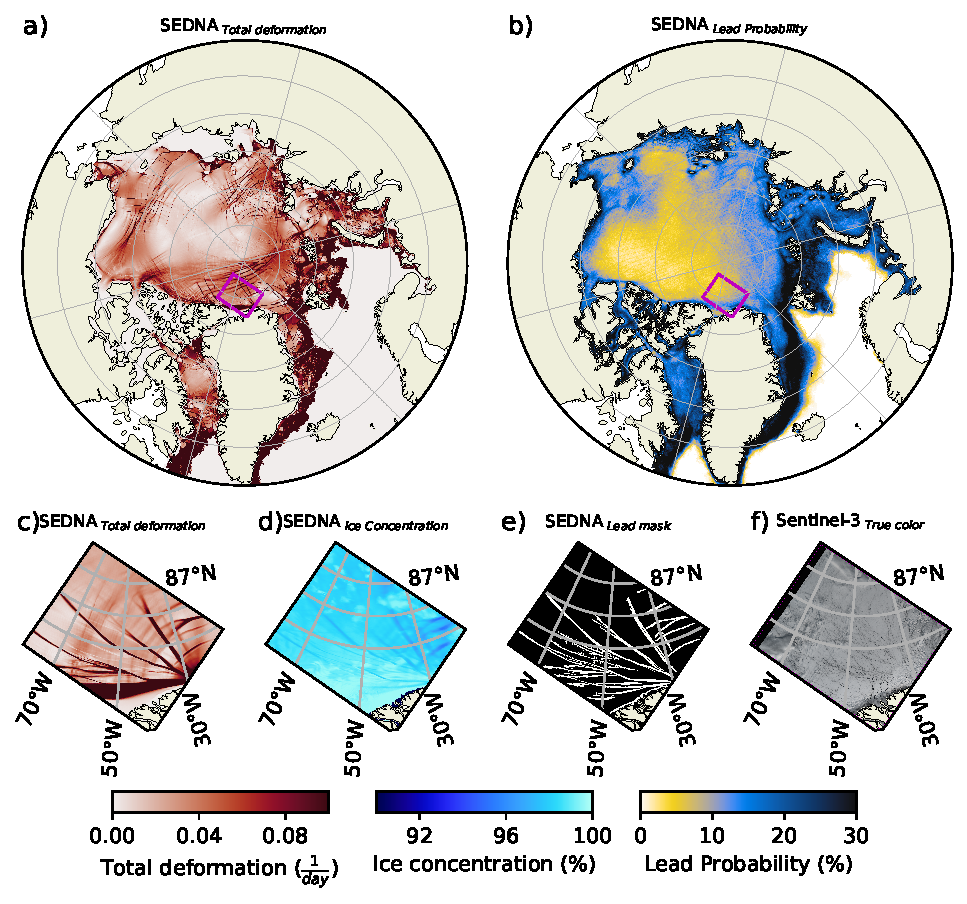
\includegraphics[width=0.95\textwidth]{./figures/Figure_1_SENTINE_SEDNA_LKF_conc_New_Color.pdf}
    \caption{a) Snapshot of total deformation for the 21st of April 2014 from SEDNA. b) Mean lead probability between 2011 and 2015 from SEDNA. c) True color image from Sentinel 3 on the 12th of April 2022 for the magenta area in panel a. d) Snapshot of the ice concentration from SEDNA on the 21st of April 2014. e) Total deformation to identify leads and f) identified mask of leads on the 21st of April 2014 in SEDNA.}
    \label{fig:fig1}
\end{figure}

To accurately represent the spatial distribution of fluxes across leads, climate models need resolutions in the subkilometer range, that they currently lack in order to resolve the localized nature of fluxes through leads \citep{Bouchat_sea_ice_rheology_2022, Wang_leads_2016}. To overcome this, here we analyse model outputs from the ocean-sea ice model SEDNA, with a resolution of $\sim 800m$ on average across the Arctic capable to capture the observational lead width distribution ($>1km$; \citealp{Wernecke_Lead_2015}). 
A snapshot of the total deformation is shown in figure \ref{fig:fig1}a.  A closer examination, focusing north of Greenland in panels c, d, e, and f of figure \ref{fig:fig1}, reveals similarities between the spatial pattern of typically observed leads on the 12th of April 2022 from a true color satellite image (Fig. \ref{fig:fig1}c) and the ice concentration of SEDNA for the 21st of April 2014. Note that the sea ice concentration in the identified leads shown in figure \ref{fig:fig1}f using the lead identification algorithm proposed by \citet{Hutter_identification_2019} remains higher than 90\% concentration; this is a consequence of continuous nature of the sea ice model and the daily averaged output that smooths the presence of leads in the fields. 
Despite the high sea ice concentration, SEDNA is capable to resolve intensified localized sea ice deformation. 

The climatology of the lead probability, i.e. the likelihood of a leads occurring for any given day, is shown in figure \ref{fig:fig1}b. The mean probability of leads averaged over the Arctic is $\sim 19\%$ in SEDNA, comparable to observations using RADARSAT Geophysical Processor System and Thermal-Infrared Satellite Imagery \citep{Wernecke_Lead_2015,Willmes_leads_currents_2023}. Although observations use different identification methods compared to the one implemented in SEDNA \citep{Hutter_identification_2019}, there is resemblance between the spatial patterns of SEDNA and observations (Fig. \ref{fig:S_fig1}). For example, we observe increased lead probability over the shelves, along bathymetric features, and in regions with large kinetic energy (Fig. \ref{fig:S_fig1}). Several hotspots of lead probability can be identified in the Chukchi Sea, highlighting the model's ability to reproduce leads dynamics. SEDNA reproduces the patterns observed in the Arctic shelves, the Greenland Sea, Barents Sea, Kara Sea and Laptev Sea, but the pattern in the Beaufort Sea in observations is not fully captured in SEDNA. Regardless, the similarities between the observations and model lead probability allow us for the first time to estimate quantitatively the impact leads have on the surface buoyancy of the Arctic Ocean.

Figure \ref{fig:fig2}a and b show two snapshots of the buoyancy flux at the ocean surface, where the haline contribution to the buoyancy flux is larger than the thermal contribution. A negative buoyancy flux in winter results mainly from sea ice refreezing and brine rejection, while, in summer, a positive buoyancy flux is associated with sea ice melting and freshening of the Arctic surface. Inside the ice covered region (magenta contour) in figure \ref{fig:fig2}, the fluxes are spatially homogeneous, except for the marginal ice zone and within the leads, where the buoyancy fluxes are larger than those underneath the ice covered ocean excluding leads. The mean flux across the Arctic for the leads is $-2.46\times 10^{-8} m^2/s^3$ and $7.20\times 10^{-8} m^2/s^3$ for each date, respectively, compared to the $-2.42\times 10^{-8} m^2/s^3$ and $5.89\times 10^{-8} m^2/s^3$ excluding the leads. In other words, on the 1st of January (winter), the total fluxes within the leads and those not in leads are comparable. However, on the 25th of June (summer), the fluxes in the leads can be up to 20\% larger than those excluding the leads.

\begin{figure}
    \centering
    
\includegraphics[width=1\textwidth]{./figures/Figure_2_buoyancy_flux_maps_vertical_V2_15p.pdf}
    \caption{Maps of buoyancy flux and transects for the 1st of January and 25th of June 2014. a) Map of buoyancy flux on the 1st of January 2014. 
    Transect on the 1st of January 2014 of c) downward heat flux, e) minus freshwater flux, g) ice thickness and i) buoyancy flux (heat flux minus freshwater flux). b) Map of buoyancy flux on the 25th of June 2014. Transect on the 25th of June 2014 of d) downward heat flux, f) minus freshwater flux, h) ice thickness and j) buoyancy flux. Note that positive buoyancy fluxes correspond to buoyancy loss, while negative buoyancy fluxes correspond to buoyancy gain. The transect location and orientation changes between the winter and summer dates. Magenta contour in panels a and b correspond to the 15\% concentration contour of sea ice. Vertical blue bars shows the mask of leads in the transect.}
    \label{fig:fig2}
\end{figure}

Two transects across the Beaufort Gyre are shown in figure \ref{fig:fig2} for the 1st of January 2014 and 25th of June 2014.
Examining the transect on 1st of January 2014, we notice that along the transect we two leads (vertical blue bars). Within these detected leads there is a significant decrease in sea ice thickness of $\approx 25cm$ and suggests an opening of the sea ice cover (Fig.\ref{fig:fig2} c).
Along this transect there is an overall small heat flux at the ocean surface and within the identified leads (Fig.\ref{fig:fig2} e), since the ocean surface is at freezing point. Thus, the extra heat exchanged with the atmosphere is used to form sea ice instead of further cooling the ocean, resulting in a heat flux close to zero at the ocean surface.
In contrast, the freshwater flux (Fig.\ref{fig:fig2}g) exhibits two prominent positive peaks, located within the identified leads where the sea ice thickness decreases. Both of these peaks are twice the magnitude of those where no leads were identified, due to an enhanced sea ice growth and brine rejection within the leads. 
The heat flux minus the salt flux result in a negative buoyancy flux for this snapshot where the largest buoyancy loss occurs within the leads (Fig.\ref{fig:fig2} i).
On the 25th of June (Fig.\ref{fig:fig2}d), we detect several leads, but not all of them show a decrease of the sea ice thickness of more than $1m$ (Fig.\ref{fig:fig2} h). The leads with a sea ice thickness decrease also experience an increase in the heat fluxes, reaching up to $\sim 25 W/m^2$ (Fig.\ref{fig:fig2}f) and a local decrease of the the freshwater flux, indicating a freshening of the surface due to sea ice melt. This change is captured by the positive buoyancy flux, decreasing the density at the surface (Fig.\ref{fig:fig2}j). Note that some peaks in the buoyancy flux align with the edge of the detected leads, likely due to the enhanced refreezing or melting that occurs at the edge of the lead. 
Of all the identified leads, some exhibit significant fluxes at the ocean surface, while others have little to no imprint in the thickness and fluxes. Detected leads  without changes in the thickness or ocean surface fluxes may be explained by the timing of the sea ice break up (divergence), where later snapshots show an increase of fluxes at the location of these identified leads (not shown). Alternatively, lead generated through shear and convergence have a limited flux exchange with the atmosphere, but may have enhanced fluxes in the ocean interior due to isopycnal upwelling/downwelling forced by the atmosphere-ocean stress within the leads \citep{Bourgault_flux_lkf_2020}.

Similar to observations, we identify fluxes that are larger in the leads than in the regions without leads for both summer and winter days. However, the freshwater flux, attributable to melting and freezing, is significantly larger than the heat fluxes associated with the leads. In the next section, we explore the spatially averaged contribution of leads in the surface the buoyancy fluxes and the integrated influence on the water mass transformation across the Arctic Basin during 2014. This analysis is conducted separately for the marginal ice zone (MIZ; 0-80\% sea ice concentration), ice pack (80-100\% sea ice concentration) and the leads within each of these regions. 


\section{Mean contribution of leads in the surface Arctic buoyancy}\label{sec3}

The ice covered Arctic experiences two main dynamical sea ice regimes, thus we split the ice covered Arctic into four distinct masks representing the MIZ, the ice pack, the leads in the MIZ, and the leads in the ice pack. The averaged percentage area of these distinct masks during 2014 is as follows: 19\% for the MIZ, 81\% for the ice pack, 14\% for the LKFs in the ice pack, and 10\% for the leads in the MIZ. 
The area covered by each mask exhibits a seasonal cycle (Fig. \ref{fig:fig3}a). During summer (June, July, and August), the percentage of the ice pack cover area decreases from approximately $90\%$ to $50\%$, while the contribution of the MIZ increases from $10\%$ to approximately $50\%$. 
On one hand, the percentage of the area covered by LKFs in the ice pack peaks in winter (December, January, and February) at almost 20\% coverage over the ice pack area. On the other hand, the contribution of the leads in the MIZ peak in summer, covering up to 25\% of the total ice cover Arctic and 50\% of the MIZ surface area. During 2014, on average the area covered by leads is $\sim 20\%$ of the total sea ice covered Arctic, consistent with previous model assessments \citep{Wang_leads_2016}. 

To quantify the contribution of the buoyancy flux occurring within the leads to the total ice covered ocean surface buoyancy flux, we integrate the buoyancy flux over each of the sea ice cover masks (Fig. \ref{fig:fig3}b), where the extent of each ice cover mask evolves temporally following the seasonal cycle of the sea ice extent. The buoyancy flux shows a significant seasonal cycle, where positive values correspond to surface waters becoming lighter due to sea ice melting and negative values to surface waters becoming denser due to sea ice formation.
The mean buoyancy flux under the ice pack in winter (December-February) and summer (June-August) is -0.33$m^2/s^3$  and 0.35$m^2/s^3$, respectively. The buoyancy flux underneath the ice pack changes sign during the seasonal cycle, suggesting a shift from ice formation in winter to ice melting in summer, dominated by the haline buoyancy component. Meanwhile, the mean buoyancy flux in the MIZ increases from -0.01$m^2/s^3$ in winter to 0.26$m^2/s^3$ in summer. The MIZ has predominantly a positive buoyancy flux suggesting preferential melting over the year, where both thermal and haline component of the buoyancy flux play a role in determining the buoyancy flux. In both, the MIZ leads and the ice pack leads, the buoyancy flux follow the same seasonality as the fluxes underneath the ice covered MIZ and ice pack.  Winter values are -0.05$m^2/s^3$ and -0.01$m^2/s^3$, while summer values reach 0.07$m^2/s^3$ and 0.14$m^2/s^3$ for the ice pack and the MIZ, respectively.
In other words, the flux within the leads accounts for between 15-20\% of the total buoyancy fluxes underneath the ice pack and between 20-50\% of the total buoyancy fluxes underneath the MIZ over the year, equivalent to their area coverage in both regions.
Moreover, the area weighted buoyancy fluxes in figure \ref{fig:fig3}c show that winter leads in the MIZ and the summer leads in the ice pack exhibit larger buoyancy fluxes per unit of area compared to those in the MIZ and ice pack, respectively. 
The mean winter buoyancy flux of the leads in the MIZ is 
-0.19 $\times10^{-7} m^2/s^3$ per $km^2$, representing a 40\% larger buoyancy flux in winter within the leads compared to those in outside the leads (-0.12 $\times10^{-7} m^2/s^3$ per $km^2$), suggesting more freezing within the leads compared to those underneath the ice-covered MIZ and ice pack. This is consistent with previous results showing larger fluxes and enhanced freezing within leads in winter \citep{Boutin_rheology_2023}. 
The mean summer buoyancy flux within the leads in the ice pack is 0.72$\times10^{-7} m^2/s^3$ per $km^2$, approximately 20\% more buoyancy flux in summer compared to the ice pack (0.59$\times10^{-7} m^2/s^3$ per $km^2$), indicating enhanced melting within the ice pack leads. 

\begin{figure}
    \centering
    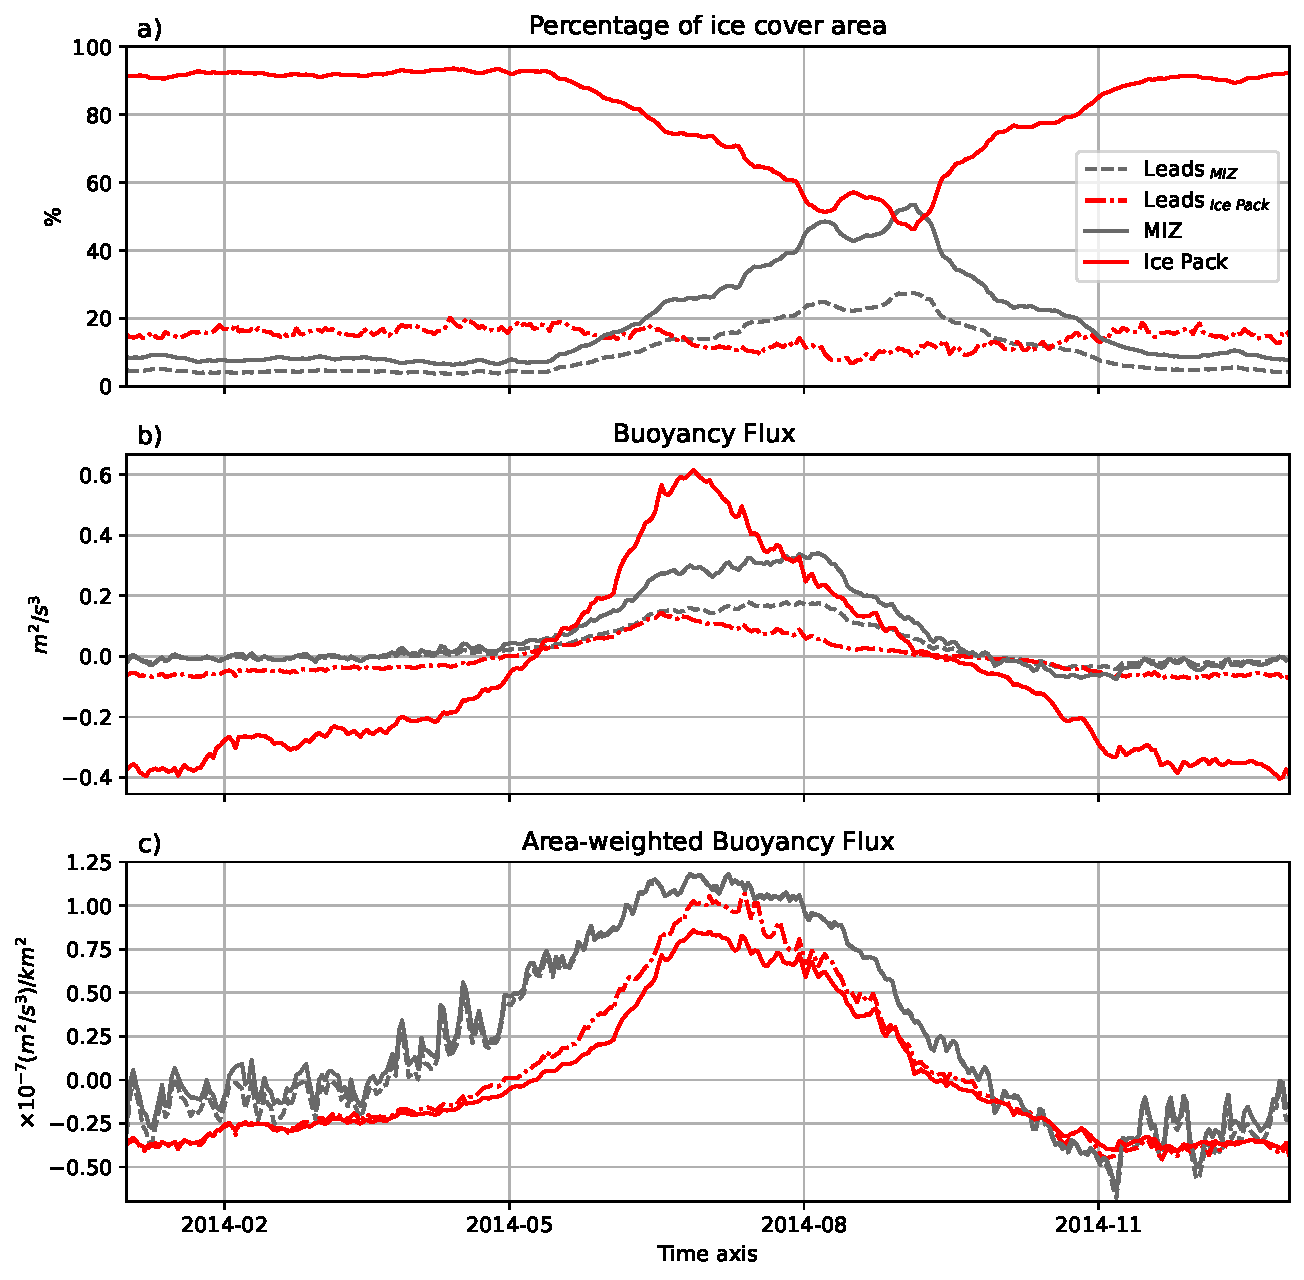
\includegraphics[width=0.9\textwidth]{./figures/Figure_3_buoyancy_flux_components_ts.pdf}
    \caption{Time-series during 2014 of a) the area cover, b) integrated buoyancy fluxes, and c) area-weighted buoyancy fluxes for the ice pack, the MIZ, and the leads in the ice pack and in the marginal ice zone. The marginal ice zone is defined between ice concentration of 0-80\%, and the ice pack is defined where ice concentration $>80\%$.}
    \label{fig:fig3}
\end{figure}

To further quantify the role and impact leads have on the surface water masses of the Arctic, we use the surface water mass transformation framework (WMT; see methods section; \citealp{Walin_WMT_1982}). This approach provides information on the transport of water through the surface density contours due to surface buoyancy forcing that results in the formation of lighter or denser water at the surface. Thus, the WMT relates the surface buoyancy to properties in the ocean interior. 
In figure \ref{fig:fig4}a, the averaged WMT during 2014 is shown for the ice covered Arctic, the ice pack, the MIZ, and the parts of these regions covered by leads. The ice-covered water mass transformation of SEDNA, including the WMT of the ice pack and the WMT of the MIZ, is consistent with previous estimates of the surface Arctic WMT \citep{Pemberton_WMT_2015}.
The yearly mean WMT in the ice pack is characterized by a broad region of strong positive transformation (losing buoyancy) corresponding to the halocline polar surface water ($PSW_{H}$; $24.36 kg/m^3 < \rho < 27.41 kg/m^3$), reaching a maximum of $\sim 2.1 Sv$.
The yearly mean WMT in the ice pack leads also features a positive peak within the $PSW_{H}$ reaching up to $0.39 Sv$. On average the WMT in the ice pack leads accounts for $\sim 10\%$ of the WMT of the ice pack. The MIZ mean WMT is mostly negative within the density range of $20 kg/m^3 < \rho < 27.5 kg/m^3$ (gaining buoyancy), reaching a minimum of $-1.2 Sv$ around $\rho = 27 kg/m^3$.  The MIZ leads WMT is also negative within the same range of densities, with a minimum of $-0.6 Sv$. On average, the WMT in the MIZ leads corresponds to $\sim 50\%$ of the WMT of the MIZ. Maps of the surface density (Fig.\ref{fig:S_fig3}) show that water mass transformation are localized geographically; the transformation of $PSW_{H}$ occurs primarily within the Eurasian basin and a smaller contribution in the Chukchi sea, the $PSW_{ML}$ ($\rho < 24.36 kg/m^3$) occurs in the Canadian basin, and the $PDW$ and $AW$ ($27.41 kg/m^3 < \rho < 27.81 kg/m^3$ and $27.81 kg/m^3 < \rho$, respectively) occurs in the Barents and Kara seas.  

Hovm\"oller diagrams of the seasonal cycle of the WMT during 2014 for the ice pack, the MIZ, and leads in each of these regions are depicted in figure \ref{fig:fig4}.
Overall, in the ice pack and MIZ, winter months show a positive transformation (loss of buoyancy), due to brine rejection during sea ice growth. Meanwhile, summer presents negative transformation or a gain of buoyancy occurs due to the melting of sea ice.  
The mean WMT underneath the ice-covered ice pack varies from 1.32 Sv in winter and -2.38 Sv in summer, and the WMT in the leads of the ice pack is 0.21 Sv in winter and -0.85 Sv in summer. In other words, the WMT in the ice pack leads explain between 20 to 30\% of the WMT occurring in the pack over the year. In the case that leads in the ice pack acted to transformed water masses within a given density range, it would be expected to observe a different pattern in the WMT of figures \ref{fig:fig4} b and c. However, there is no evidence in the WMT ratios that leads transform particularly water masses in the ice pack (Fig. \ref{fig:fig4} g). In fact, ice pack leads transform the same water masses as those transformed underneath the ice-covered ice pack. The WMT in MIZ leads in summer is comparable to the summer MIZ WMT.  In winter MIZ leads transform -0.58 Sv, approximately 50\% of the winter MIZ WMT (-1.1 Sv). Similarly to the leads in the ice pack, there is no evidence of leads in the MIZ to transform different water masses to those underneath the ice-covered MIZ. 
Adding all the leads in the Arctic, those in the MIZ and the ice pack, they contribute between 20-35\% of the WMT throughout the year, again a contribution comparable to the area covered by leads in the ice covered Arctic. 

\begin{figure}[!ht]
    \centering
    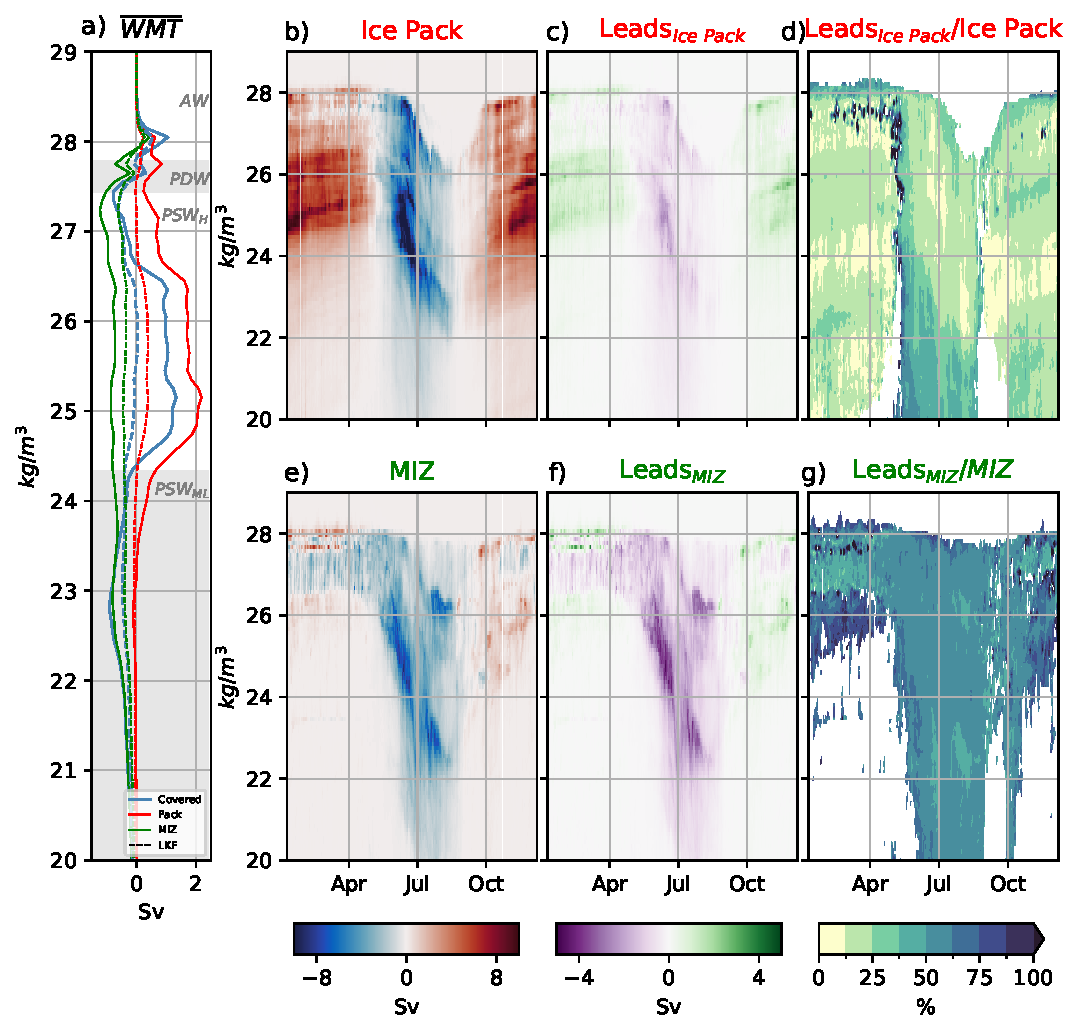
\includegraphics[width=1\textwidth]{./figures/Figure_4_water_mass_transformation_hovmoller_V2.pdf}
    \caption{Mean and daily Water mass transformation over 2014. a) Mean water mass transformation over 2014 for the ice pack, MIZ, and leads in each region. Hovmoller diagram of the water mass transformation (Sv) for the b) ice pack, c) ice pack leads and d) the ratio of water mass transformation between the leads and the ice pack region.
    Panels e), f), and g) follow the same structure as panels b), c) and d), but for the MIZ, MIZ leads, and ratio between them.
    Shaded gray and white areas in panels a) represent the water masses of the Arctic ocean \citep{Pemberton_WMT_2015}: the mixed layer polar surface water ($PSW_{ML}$; $\rho < 24.36 kg/m^3$), the halocline polar surface water ($PSW_{H}$; $24.36 kg/m^3 < \rho < 27.41 kg/m^3$), the polar deep water ($PDW$; $27.41 kg/m^3 < \rho < 27.81 kg/m^3$), and the Atlantic water ($AW$; $27.81 kg/m^3 < \rho$).}
    \label{fig:fig4}
\end{figure}

\section{Conclusions}

Leads are ubiquitous in the sea ice covered oceans and they allow exchanges between the ocean and the atmosphere and enhance locally melting and freezing of sea ice. Generally, the importance of these fluxes at the ocean surface are considered to be of significant importance for the Arctic dynamics \citep{Maykut_solar_1995}. The present study assesses the impact of leads in the ocean surface by diagnosing the buoyancy fluxes using a very high-resolution hindcast (SEDNA). The lead identification algorithm implemented in SEDNA allows us to reproduce the observed leads spatial distribution over most regions of the Arctic, with exception of the Beaufort Sea. However, the identification algorithm, time periods, and the spatial and temporal scales used are different between the present study and that of \citealp{Willmes_leads_currents_2023}.  Despite these regional differences, SEDNA can estimate the mean lead probability, showcasing its capacity to capture the dynamics of these features. This high resolution simulation allows us to better understand the role of leads in shaping the buoyancy fluxes of the Arctic ocean.

Using SEDNA, we found that leads cover $\sim 20\%$ of the sea-ice covered Arctic, and in the ice pack, leads can contribute up to 20\% more buoyancy flux compared to the fluxes outside the leads. Despite these larger buoyancy fluxes, leads only account for approximately $\sim 20\%$ of the total surface water mass transformation in the ice covered Arctic, which is roughly equivalent to their area coverage. Thus, contrary to previous hypotheses, our findings suggest that leads have a smaller contribution to the transformation of surface water masses in the Arctic Ocean than previously thought (e.g. \citealp{Hutter_identification_2019, McPhee_LKF_2005}). While their presence can induce localized changes in the density of surface waters due to brine rejection and ice melting, their spatial extent and duration are not sufficient to significantly alter the water masses. Thus revealing that leads are likely unable to imprint a signal in the interior of the Arctic Ocean, since fluxes are too weak, the water mass transformation volume is insufficient and the halocline is too strongly stratified to penetrate the base of the mixed layer \citep{Lenn_mixing_2022}.
Furthermore, the transformation of water masses in the leads have the same sign and magnitude as those underneath the surrounding ice-covered regions (excluding leads). Thus, there is no evidence that leads act differently or that they have a particular imprint on the Arctic ocean water masses.

Here we focus on the surface forced WMT, but further studies are required to assess the impact of process resulting from leads in the mixed layer and the ocean interior, such as WMT due to enhanced mixing within leads, the upwelling of isopycnals through Ekman pumping \citep{McPhee_LKF_2005}, the impact of entrainment in the mixed layer within the leads, the source of potential energy and generation of mixed layer instabilities due to isopycnal tilting in the vicinity of leads. For example, in SEDNA we note that the mixed layer depth (MLD) is shallower in leads than the regions outside the leads (Fig.\ref{fig:S_fig2}). Although, this difference in MLD is significant and, on average, the MLD is $\sim 20\%$ shallower during winter in the ice pack leads, there is no evidence of an impact in the ice cover nor a distinct response to the surface buoyancy fluxes or change of the water mass transformation within these leads. A limitation of this study is the use of a continuous sea ice model that results in leads with high ice thickness and concentrations, thus limiting the exchanges between the ocean and the atmosphere. In contrast, future studies using floe resolving models that allow more ``realistic leads" with direct exchanges between the ocean an the atmosphere would likely result in larger fluxes through the leads increasing their potential impact in the water mass transformation and ocean mixed layer.

Leads have an important local effect in the atmosphere and the sea-ice fluxes \citep{Lupkes_leads_2008,Marcq_flux_lead_2012, Wettlaufer_insulator_1997, Smith_polynyas_1990}, but a limited imprint in the ocean fluxes. Our results suggest that leads are not the first order mechanism controlling the water mass transformation at the surface, thus having a minor impact in the stratification and surface layer dynamics of the Arctic Ocean.
Therefore, resolving and/or parameterizing leads in climate models are likely to have a negligible impact improving the well known issue within the Arctic climate modeling community of the misrepresentation of the stratification and water masses in the Arctic ocean \citep{Wang_ompi_2024,Ilicak_core_2016}. Finally, the probability of leads to occur in the ice pack has been projected to increase as the Arctic sea ice transitions towards thinner, younger, and more mobile sea ice \citep{Boutin_rheology_2023, IPCC_arctic_2022}. Our results focus in one year and the future impact of more abundant leads is not represented in our simulations. Thus, dedicated studies are required to better estimate the surface buoyancy forcing within leads in the context of an evolving Arctic Ocean.  

\section{Methods}
\subsection*{Model description}

Here we employ the NEMO numerical platform (release 4.0.5; \citealp{NEMO_man}) to establish a 1/60$^\circ$ pan-Arctic ocean-sea ice configuration named SEDNA. The ocean core (NEMO-OPA) solves the primitive equations using finite differences on an Arakawa C-grid mesh, and it is coupled to the SI3 sea-ice component (NEMO-SI3; \citealp{SI3_man}). The pan-Arctic domain covers the Bering Strait on the Pacific side and extends southward to 56$^\circ$N in the Subpolar North Atlantic gyre and to the Baltic Sea entrance. The ocean model incorporates a linear free surface, utilizes a 3rd order flux form scheme for momentum advection, and employs a 4th order Flux Corrected Transport (FCT) for tracer advection. Additionally, the sea-ice representation uses an Elasto-Visco-Plastic (EVP) rheology with 5-categories of sea ice thickness distribution and a land-fast parameterization to better simulate sea-ice behavior above shelves.

The NCAR bulk formula from \citet{Large_global_2009} to calculate air-sea fluxes and uses hourly ERA5 atmospheric data for near-surface variables \citep{Hersbach_ERA5_2020}. The three lateral boundaries are constrained with daily GLORYS12V1 Re-analysis data \citep{GLORYS12}. Monthly freshwater fluxes from river discharges are combined with Greenland land ice melt data \citep{HuEA_rivers_2019}. The simulation extends over seven years (2009 to 2015) and starts from rest, utilizing initial conditions based on the World Ocean Atlas 2009 temperature/salinity and mean January 2009 ice state from PIOMAS re-analysis \citep{levitus_ocean_2010, PIOMAS}. Preliminary assessment against available observations and re-analyses data shows that the simulation reasonably captures key ocean and sea-ice characteristics.


\subsection*{Identification of leads}

The leads from SEDNA are identified by using the algorithm proposed by \citet{Hutter_identification_2019}. This method uses the total deformation rate defined as: 
\begin{equation}
    T_d = \left[\left(\underbrace{\frac{\partial u}{\partial x} +\frac{\partial v}{\partial y}}_{Divergence}\right)^2 + \underbrace{\left(\frac{\partial u}{\partial x} - \frac{\partial v}{\partial y}\right)^2+ \left(\frac{\partial u}{\partial y} + \frac{\partial v}{\partial x}\right)^2}_{Shear}\right]^{1/2},
\end{equation}
where $u$ and $v$ are the sea ice velocities. The deformation rate varies spatially depending on the background deformation and the sea ice properties \citep{Reiser_LKF_2020}, where the largest deformation rates occur along the boundaries of ice floes where the leads are found. Therefore, to identify the leads, the local maxima is identified using a difference of Gaussian filter (DoG filter) of the deformation rate field. After this, a binary map is created with the mask of identified lead. Note that after this step, \citet{Hutter_identification_2019} reduce the leads width to a line to then track the leads over time. Since our study focus on the ocean-atmosphere interactions, we only use the identification algorithm to produce a mask of leads during 2014 for the Arctic, thus we retain the original lead width computed from the deformation rate. Finally, the lead mask is then used to quantify and contrast the impact of leads compared to the ice covered Arctic, the ice-pack (ice concentration $> 80\%$) and the MIZ (0 - 80\% ice concentration).

\subsection*{Buoyancy flux and water mass transformation}
 
Heat fluxes (heating and cooling) and freshwater fluxes (evaporation, precipitation, runoff, and sea ice melt/growth) at the ocean surface result in a buoyancy forcing capable to change the density of the surface seawater. Here, the buoyancy flux is computed as:

\begin{equation}
    B_f = \underbrace{\frac{g \alpha Q_{net}}{\rho_0 C_p}}_{Net\ surface\ heat\ flux} - \underbrace{\frac{g \beta F_{net} SSS }{\rho_0}}_{Net\ surface\ freshwater\ flux},
\end{equation}

where $Q_{net}$ the net heat flux at the sea surface, $\alpha$ the thermal expansion coefficient, $SSS$ the sea surface salinity, $F_{net}$ the net fresh water flux that includes evaporation, precipitation, runoff, and freezing minus melting flux, and $\beta$ the haline contraction coefficient. With constant values of $g = 9.81 m/s^2$ and the ocean density $\rho_0 = 1026 kg/m^3$. 
Note that using this sign convention, positive values in the buoyancy forcing decrease the surface density making the ocean surface more buoyant (stable) and negative values increase the surface density. 

\citet{Nurser_WMT_1999} and  \citet{Walin_WMT_1982} proposed the water mass transformation framework that quantifies the rate at which a given water mass is made lighter (negative transformation rate) or denser (positive) due to surface fluxes. The surface water mass transformation is computed as:

\begin{equation}
    \Omega(\sigma_k) = \underbrace{- \frac{1}{\sigma_{k+1}-\sigma_k}\iint_A\left(\frac{\alpha Q_{net}}{\rho_0 C_p}\right)dA}_{Net\ surface\ heat\ flux} + \underbrace{\frac{1}{\sigma_{k+1}-\sigma_k}\iint_A\left(\frac{\beta F_{net} SSS }{\rho_0}\right)dA}_{Net\ surface\ freshwater\ flux},
\end{equation}

where $\sigma$ is potential density and the indices $k$ represents the density bin number. The transformation rate $\Omega$ is spatially decomposed into different sea-ice dynamics such as the ice covered, the pack ice, the MIZ, and the leads in each of these regions. 
%By separately diagnosing the density transformation that occurs in the leads and underneath the surrounding floes, we quantify the relative importance of the leads for each of these regions. Additionally, this framework accounts for the area changes of the ice cover during the seasonal cycle, and excludes open ocean regions.

\backmatter

\bmhead{Open Source}

The SEDNA model configuration are described and publicly available at \url{https://zenodo.org/records/7656924}.
All analyses and figures in this manuscript are reproducible via Jupyter notebooks and instructions can be found in the GitHub repository \texttt{Leads\_Arctic\_ocean} (\url{https://github.com/josuemtzmo/Leads_Arctic_ocean}).

\bmhead{Acknowledgements}

We acknowledge funding from the ANR ImMEDIAT project (ANR-18-CE01-0010) and the MEDLEY project funded by the program JPI Ocean/JPI Climate (ANR-19-JPOC-0001) project. Analyses were undertaken on the Datarmor, IFREMER in Brest in conjunction with Joliot-Curie at GENCI\makeatletter@CEA granted by PRACE with computing resources of 35 Million core hours.


%%===========================================================================================%%
%% If you are submitting to one of the Nature Portfolio journals, using the eJP submission   %%
%% system, please include the references within the manuscript file itself. You may do this  %%
%% by copying the reference list from your .bbl file, paste it into the main manuscript .tex %%
%% file, and delete the associated \verb+\bibliography+ commands.                            %%
%%===========================================================================================%%

%% if required, the content of .bbl file can be included here once bbl is generated
%%\input sn-article.bbl


\bibliography{biblio}


\pagebreak

\begin{appendices}

\renewcommand{\thefigure}{S\arabic{figure}}

\begin{figure}
    \centering
    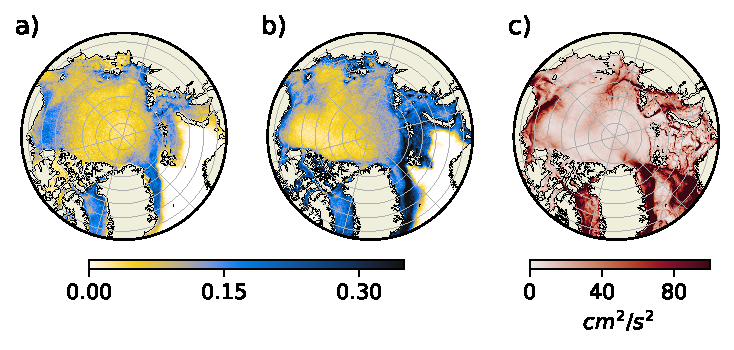
\includegraphics[width=1\textwidth]{./figures/comparison_LKF_observations_KE.pdf}
    \caption{Comparison of winter lead frequency between a) Thermal-Infrared Satellite Imagery \citep{Willmes_leads_currents_2023} and b) SEDNA between 2011 and 2015. Panel c) shows the SEDNA mean kinetic energy between 2011 and 2015.}
    \label{fig:S_fig1}
\end{figure}

\begin{figure}
    \centering
    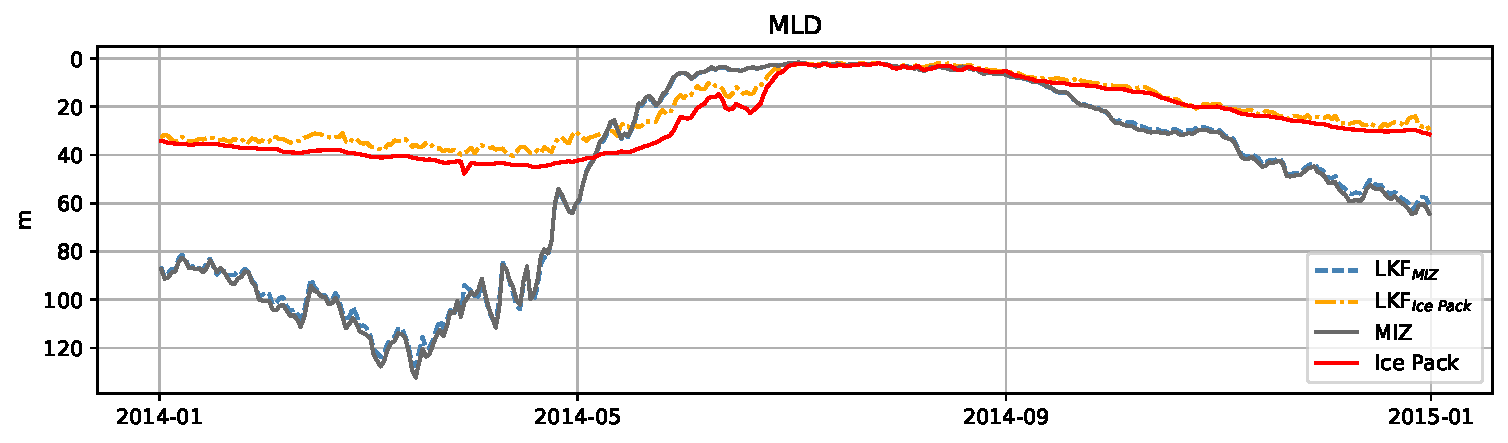
\includegraphics[width=1\textwidth]{./figures/Figure_S2_TS_MLD.pdf}
    \caption{Time-series during 2014 of the mean mixed layer depth for linear kinematic features in the ice pack, the linear kinematic features in the marginal ice zone, the marginal ice zone (ice concentration 0-80\%), and the ice pack (ice concentration $>80\%$). The mixed layer depth is defined as the 0.1 density anomaly referenced to the first ocean model level.}
    \label{fig:S_fig2}
\end{figure}

\begin{figure}
    \centering
    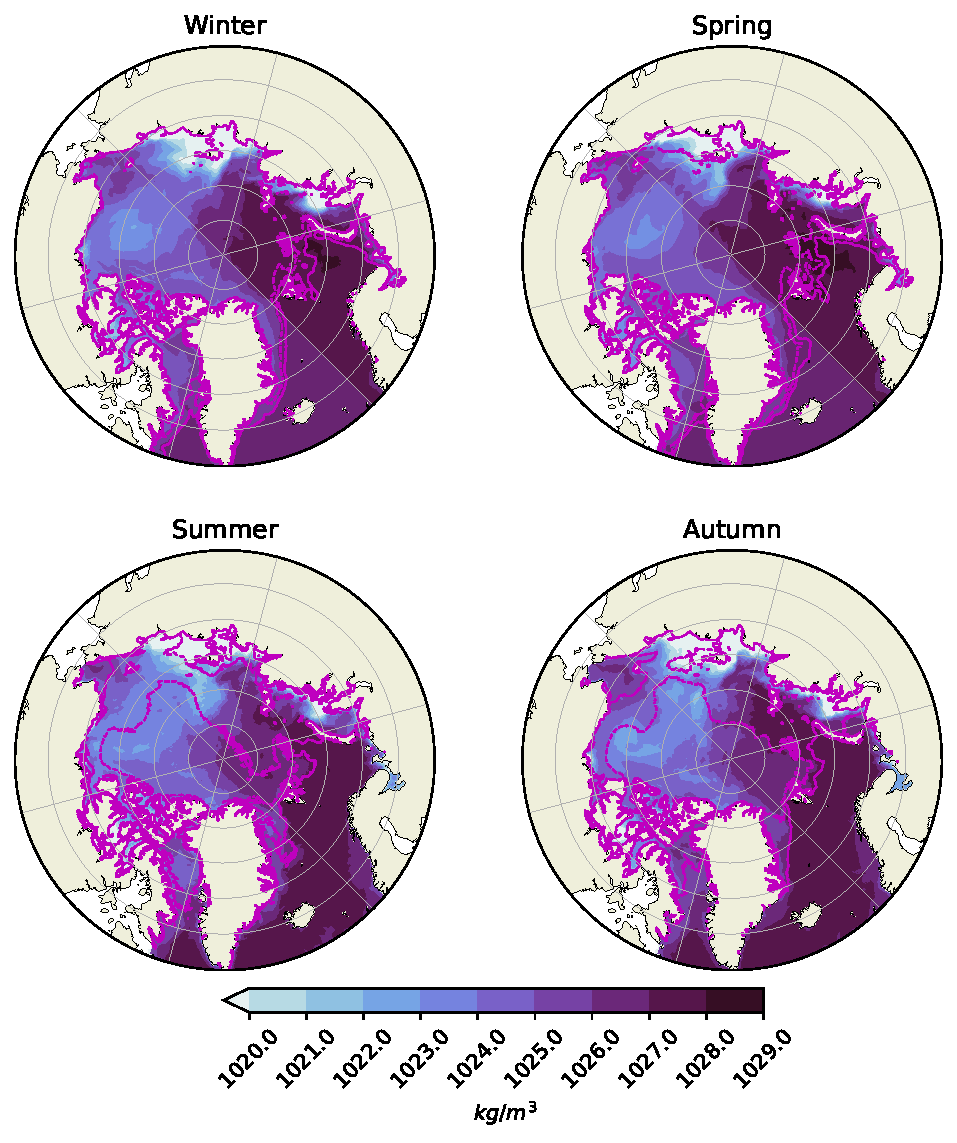
\includegraphics[width=1\textwidth]{./figures/Figure_S1_density_maps_season.pdf}
    \caption{Maps of the seasonal surface density of SEDNA during 2014. Solid and dashed magenta contour in maps correspond to the 0\% and 80 \% concentration contour of sea ice respectively.}
    \label{fig:S_fig3}
\end{figure}

\end{appendices}

\end{document}
